\chapter{Background} \label{chap:background}

Natural language processing (NLP) has gained significant importance in recent
years as an area of computer science \cite{eisenstein2019intro2nlp}. NLP deals
with the processing of natural language such as English or German
\cite{hapke2019natural}. This chapter elaborates on the technical background
needed to enable a computer to understand text and solve specific tasks on
textual data. Section~\ref{sec:tokenizers} covers different tokenization
strategies and embeddings to represent the meaning of words.
Section~\ref{sec:lm} discusses the concept of language modeling, which lies at
the core of many NLP tasks, and introduces two different training objectives for
language models. Moreover, we cover the topic of Transformer-based language
models in Sec.~\ref{sec:transformers} that gave rise to most contemporary NLP
systems \cite{min2023recent}.

\section{Tokenizers and Word Embeddings} \label{sec:tokenizers}

\begin{figure}[htb]
    \centering
    \resizebox*{.8\textwidth}{!}{\usetikzlibrary {arrows.meta} 

\tikzset{
    block/.style={rectangle, draw, thick, text centered, font=\bfseries, inner sep=.4cm}
}

\begin{tikzpicture}[node distance=5.4cm]

    % Nodes
    \node (tokenization) [block] {Tokenization};
    \node (embedding) [block, right of=tokenization] {Embedding};
    
    % Arrows
    \draw[->] ++(-4, 0) -- (tokenization.west) node[midway, above] {Raw Text};
    \draw[->] (tokenization.east) -- (embedding.west) node[midway, above] {Tokens};
    \draw[->] (embedding.east) -- ++(3, 0) node[midway, above] {Embeddings};
\end{tikzpicture}
}
    \caption{Preprocessing steps in NLP}
    \label{fig:nlp_preprocess}
\end{figure}

In contrast to programming languages, natural languages that human beings use to
communicate cannot be natively understood by computers. This is due to the fact
that no compilers for human languages exist that allow translation of natural
languages into machine-interpretable languages \cite{hapke2019natural}.
Nonetheless, with certain models, natural languages can become interpretable for
machines, thus computers are able to act upon them \cite{hapke2019natural}.
Because of the good performance, neural networks have become the
state-of-the-art for NLP tasks \cite{otter2020survey}. However, neural networks
operate on continuous numerical values, so text cannot be directly processed by
these networks. Hence, the text has to be first transformed into numerical
representations as illustrated in Fig.~\ref{fig:nlp_preprocess}.

\begin{figure}[htb]
    \centering
    \begin{tikzpicture}[
    node distance=1cm,
    font=\bfseries
]

    % Nodes
    \node (text) {"This is an apple."};
    \node (tokens) [below=of text] {["This", "is", "an", "apple", "."]};
    \node (ids) [below=of tokens] {[1, 5, 103, 1027, \texttt{[EOS]}]};

    % Arrows
    \draw[->] (text) -- (tokens);
    \draw[->] (tokens) -- (ids);

\end{tikzpicture}

    \caption{Example of segmenting a sentence into word tokens}
    \label{fig:tokenization}
\end{figure}

The raw text is mapped to discrete values by applying tokenization, the process
of segmenting text into units of so-called tokens (refer to
Fig.~\ref{fig:tokenization}). The example shows a tokenization process in which
the text is split by whitespace into words. Note that tokens can not only take
the form of words, but also subwords or even sentence pieces depending on the
applied tokenization strategy. In order to transform the obtained tokens into
discrete values, tokens are mapped to indices referring to the given position in
a vocabulary, the set of all unique tokens \cite{mielke2021between}.
Furthermore, observe how the period symbol, which semantically marks the end of
a sentence has been mapped to a special \texttt{[EOS]} token. Special tokens are
a set of additional tokens in the vocabulary reserved for specific purposes
beyond regular words or subwords. These tokens are used to instruct upstream
models to perform certain tasks or to provide additional information in order to
facilitate model behavior during training and inference.

\subsubsection{Tokenization Strategies}

% Tokenization algorithms can generally be divided into two main categories:
\paragraph{Top-down tokenization} Top-down or \textit{rule-based} algorithms
involve establishing a tokenization standard by defining a set of deterministic
rules and applying them to a given input string. Rules can be as simple as
splitting by whitespace and punctuation, or they can be more sophisticated such
as those used in the \textit{Penn Treebank} \cite{marcus1993building},
\textit{Moses} \cite{koehn2007moses} and \textit{spaCy} \cite{honnibal2017spacy}
tokenizers. Other rule-based approaches extend this framework by addressing the
semantic equivalence of words. For example, \textit{stemming} is a technique
that reduces inflected forms of a word to their word stem, as seen in the
transformation of 'running' and 'ran' to 'run'. 

\paragraph{Bottom-up tokenization} In modern NLP bottom-up or \textit{subword}
tokenization algorithms are more commonly used. Instead of explicitly defining
tokens through rules, these algorithms learn the tokens from the data itself by
analyzing the statistical properties of letter sequences. Learning the
characters. These characters are then iteratively merged based on, e.g.
occurrence or likelihood in the data to form tokens. As a result, the learned
tokens can consist of entire words, fragments of words, or they can be
meaning-bearing units like morphemes\footnotemark{}, e.g. \textit{un-, -er,
-ly}, which is why they are referred to as subwords. Using subwords as tokens
allows for a reduction of vocabulary size and handling of out-of-vocabulary
words by decomposing unseen words into known subwords. This is particularly
useful for languages with large vocabularies or for specialized domains with
many technical terms. Two widely used subword tokenization algorithms are
\textit{Byte-Pair Encoding} \cite{sennrich2016neural} and \textit{unigram
language modeling} \cite{kudo2018subword}. Unigram language modeling uses a
probabilistic approach to induce subwords without any merging process and is
frequently used in conjunction with \textbf{SentencePiece}
\cite{kudo2018sentencepiece}. We will introduce the \textbf{Byte-Pair Encoding}
and the closely related
\textbf{WordPiece}
\cite{schuster2012japanese} tokenizers in Sec.~\ref{subsec:bpe} and
Sec.~\ref{subsec:wordpiece}, respectively. \\

\footnotetext{A morpheme is the smallest meaning-bearing unit of a language,
e.g. the word \textit{unwashable} has the morphemes \textit{un-}, \textit{wash},
and -\textit{able}.}

Tokenization efficiency is critical as it constitutes the initial step in most
NLP applications and must be executed quickly to prevent performance
bottlenecks. The size of the vocabulary significantly influences this
efficiency, as larger vocabularies require increased processing time for input
text. Furthermore, each NLP model is composed of a tokenizer specifically
designed for that model, meaning that tokenizers are typically not
interchangeable between different models. This is due to each tokenizer inducing
its own vocabulary. Consequently, using a tokenizer from one model with another
would result in incompatible tokenized inputs, which the other model would not
be able to interpret correctly.

\subsubsection{Word Embeddings} \label{subsec:word_embeddings}

In the final step of Fig.~\ref{fig:nlp_preprocess}, the obtained tokens or more
precisely, their respective token IDs are embedded into continuous vector
representations and subsequently used as inputs for NLP algorithms (refer to
Fig.~\ref{fig:embedding}). Such word embeddings are a technique in NLP that aims
to capture the meaning of words based on their context in text. The underlying
principle of word embedding is inspired by the \textit{distributional
hypothesis}~\cite{harris1954distributional} formulated by linguists in the
1950s, which suggests that words appearing in similar contexts tend to have
similar meanings. For instance, the words \textit{king} and \textit{queen} are
more likely to co-occur in a sentence, as are \textit{Berlin} and
\textit{Germany}. This idea of word similarities has been expressed in NLP by
representing words as points in a multidimensional semantic vector space. Here,
the relative similarity between vectors, measured by cosine distance, correlates
to their semantic similarity. The authors of \cite{mikolov2013distributed} have
shown that this approach of distributed word representation in a vector space,
by grouping similar words, helps NLP algorithms to achieve better performance.

\begin{figure}[htb]
    \centering
    \tikzset{ids/.style={text width=6mm},
         vectors/.style={text width=3cm, align=center}}    

\begin{tikzpicture}[
    node distance=0.5cm,
    font=\bfseries
]
    % Nodes for each ID and corresponding embedding vector
    \node (id1) [ids] {1};
    \node (vector1) [vectors, right=2cm of id1] {[-0.76, 0.01, -0.16]};

    \node (id5) [ids, below=of id1] {5};
    \node (vector5) [vectors, right=2cm of id5] {[0.12, 0.63, -0.11]};

    \node (id103) [ids, below=of id5] {103};
    \node (vector103) [vectors, right=2cm of id103] {[0.42, 0.71, -0.89]};

    \node (id1027) [ids, below=of id103] {1027};
    \node (vector1027) [vectors, right=2cm of id1027] {[0.27, -0.12, 0.99]};

    % Arrows between IDs and embeddings
    \draw[shorten >=0.5cm, shorten <=0.5cm, ->] (id1) -- (vector1);
    \draw[shorten >=0.5cm, shorten <=0.5cm, ->] (id5) -- (vector5);
    \draw[shorten >=0.5cm, shorten <=0.5cm, ->] (id103) -- (vector103);
    \draw[shorten >=0.5cm, shorten <=0.5cm, ->] (id1027) -- (vector1027);

\end{tikzpicture}

    \caption{Example of embedding token IDs into continuous vectors}
    \label{fig:embedding}
\end{figure}

Typically, word embeddings are learned in an unsupervised manner from large
amounts of unstructured text data. Two commonly used methods are \textbf{TF-IDF}
\cite{luhn1957statistical, sparck1972statistical} and \textbf{Word2vec}
\cite{mikolov2013distributed}. The former is a statistical method that assigns a
score to each word in a document based on its frequency and importance in the
document and the corpus. Word2vec uses a shallow two-layer neural network to
produce word embeddings. The model is trained to predict the probability of a
word appearing in a context given the word itself. The embeddings are learned by
minimizing the difference between the predicted probability and the actual
probability of the word appearing in the context.

Both methods yield \textit{static embeddings}, meaning that the method learns
one fixed embedding for each word in the vocabulary. They form the basis for
more powerful dynamic or \textit{contextual embeddings}, such as those in
\textbf{BERT} (introduced in Sec. \ref{sec:bert}), in which the vector for each
word differs from context to context (refer to
Fig.~\ref{fig:context_embedding}).

\begin{figure}[htb]
    \centering
    \begin{tikzpicture}[font=\bfseries]
    \node[anchor=west] (text1) at (0, 1.5) {"A \uline{bat} is needed when playing baseball."};
    \coordinate (bat1) at ($(text1.west) + (1, -0.25)$);
    \draw[->] (bat1) -- ++(0, -0.75) -- ++(4, 0) node[anchor=west] {[-0.76, 0.27, 0.89]};

    \node[anchor=west] (text2) at (0, -0.5) {"A \uline{bat} is a nocturnal animal."};
    \coordinate (bat2) at ($(text2.west) + (1, -0.25)$);
    \draw[->] (bat2) -- ++(0, -0.75) -- ++(4, 0) node[anchor=west] {[0.81, -0.01, -0.16]};
\end{tikzpicture}

    \caption{Example of contextual embeddings with exemplary values}
    \label{fig:context_embedding}
\end{figure}

\subsection{Byte-Pair Encoding} \label{subsec:bpe}

Byte-Pair Encoding (BPE) is a subword tokenization algorithm that was introduced
in~\cite{sennrich2016neural}. It is a data-driven algorithm and expects a
training corpus for token generation as well as the desired vocabulary size as
inputs. As previously mentioned, subword tokenizers start with a base vocabulary
consisting of all individual characters that occur in the input training corpus.
The BPE token learner then determines the most frequent adjacent character
sequence and merges it to form a new token. The merging process is repeated $k$
times until the desired vocabulary size of $k$ novel tokens plus the amount of
characters in the base vocabulary is reached. Note that as such, $k$ (the number
of merges to perform) is a hyperparameter of the BPE token learner. The
resulting vocabulary is then used by the \textit{token segmenter} to tokenize
input text. 

The BPE algorithm is usually applied inside words, not merging outside of word
boundaries and thus relies on a pre-tokenizer that splits the training corpus by
whitespace into words. In the following we give an example of the BPE token
learner's operation. Consider the tiny corpus consisting of the following set of
18 words with their occurrences in the corpus (the word \textit{low} appears 5
times, the word \textit{lower} 2 times and so on), which would result in the
initial vocabulary of 10 characters:

\begin{center}
    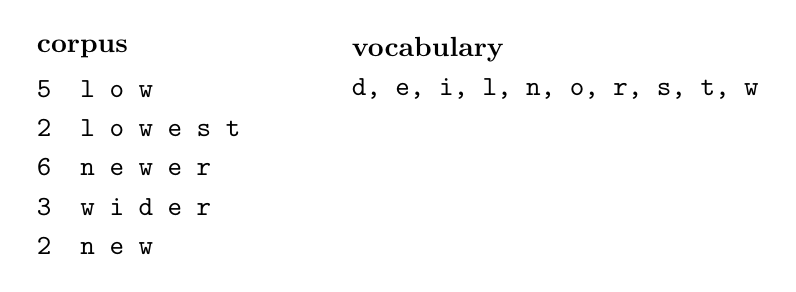
\begin{tikzpicture}[font=\ttfamily]
    % Corpus table
    \node[anchor=west, font=\bfseries] at (0, 0) {corpus};
    \node[anchor=west] at (0, -0.5) {5\quad l o w};
    \node[anchor=west] at (0, -1) {2\quad l o w e s t};
    \node[anchor=west] at (0, -1.5) {6\quad n e w e r};
    \node[anchor=west] at (0, -2) {3\quad w i d e r};
    \node[anchor=west] at (0, -2.5) {2\quad n e w};

    % Vocabulary table
    \node[anchor=west, font=\bfseries] at (4, 0) {vocabulary};
    \node[anchor=west] at (4, -0.5) {d, e, i, l, n, o, r, s, t, w};
\end{tikzpicture}

\end{center}

The BPE token learner counts the frequency of all pairs of adjacent symbols in
the vocabulary and merges the most frequent pair. In this case, the pair
\texttt{e} followed by \texttt{r} is the most frequent with a count of $6 + 3 =
9$. The first merge rule the tokenizer learns is to treat the pair \texttt{(e,
r)} as a single token, which is subsequently added to the vocabulary. The set of
words and vocabulary is updated as follows:

\hspace{2cm} 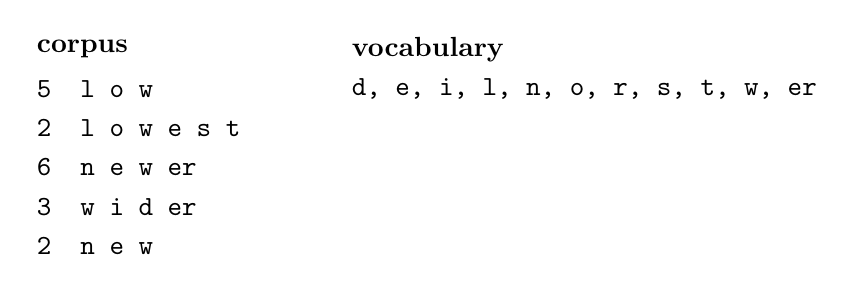
\begin{tikzpicture}[font=\ttfamily]
    % Corpus table
    \node[anchor=west, font=\bfseries] at (0, 0) {corpus};
    \node[anchor=west] at (0, -0.5) {5\quad l o w};
    \node[anchor=west] at (0, -1) {2\quad l o w e s t};
    \node[anchor=west] at (0, -1.5) {6\quad n e w er};
    \node[anchor=west] at (0, -2) {3\quad w i d er};
    \node[anchor=west] at (0, -2.5) {2\quad n e w};

    % Vocabulary table
    \node[anchor=west, font=\bfseries] at (4, 0) {vocabulary};
    \node[anchor=west] at (4, -0.5) {d, e, i, l, n, o, r, s, t, w, er};
\end{tikzpicture}


Next the pair \texttt{(n, e)} with a total count of 8 is merged into the new
token \texttt{ne}:

\hspace{2cm} 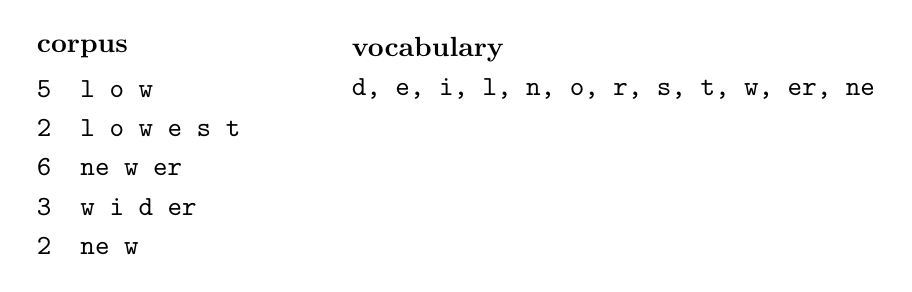
\begin{tikzpicture}[font=\ttfamily]
    % Corpus table
    \node[anchor=west, font=\bfseries] at (0, 0) {corpus};
    \node[anchor=west] at (0, -0.5) {5\quad l o w};
    \node[anchor=west] at (0, -1) {2\quad l o w e s t};
    \node[anchor=west] at (0, -1.5) {6\quad ne w er};
    \node[anchor=west] at (0, -2) {3\quad w i d er};
    \node[anchor=west] at (0, -2.5) {2\quad ne w};

    % Vocabulary table
    \node[anchor=west, font=\bfseries] at (4, 0) {vocabulary};
    \node[anchor=west] at (4, -0.5) {d, e, i, l, n, o, r, s, t, w, er, ne};
\end{tikzpicture}


Assuming a desired vocabulary size of 15, i.e. $k = 5$, the remaining merge
rules are:

\begin{center}
    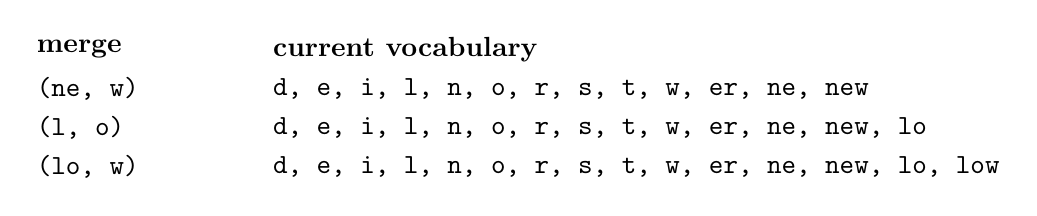
\begin{tikzpicture}[font=\ttfamily]
    % Column titles
    \node[anchor=west, font=\bfseries] at (0, 0) {merge};
    \node[anchor=west, font=\bfseries] at (3, 0) {current vocabulary};
    
    % First row
    \node[anchor=west] at (0, -0.5) {(ne, w)};
    \node[anchor=west] at (3, -0.5) {d, e, i, l, n, o, r, s, t, w, er, ne, new};

    % Second row
    \node[anchor=west] at (0, -1) {(l, o)};
    \node[anchor=west] at (3, -1) {d, e, i, l, n, o, r, s, t, w, er, ne, new, lo};

    % Third row
    \node[anchor=west] at (0, -1.5) {(lo, w)};
    \node[anchor=west] at (3, -1.5) {d, e, i, l, n, o, r, s, t, w, er, ne, new, lo, low};

\end{tikzpicture}

\end{center}

The resulting vocabulary and merge rules constitute the final BPE tokenization
model. To tokenize an input text, the merge rules are applied greedily in the
order they were learned by replacing the merged pairs with the corresponding
token. For example, the word \textit{lower} would be split into the two tokens
\texttt{low} and \texttt{er}. But a known word from the training corpus like
\textit{new} is tokenized as a full word \texttt{new}. In a real setting, BPE is
trained on a very large input corpus producing thousands of merge rules with a
vocabulary size of around 32,000 to 64,000. The result is that most words will
be represented as single tokens, and only rare and unknown words will be
tokenized by subwords while maintaining a manageable vocabulary size. This
behavior emphasizes BPE tokenization's more balanced approach to language
modeling, serving as a middle ground between character and word-level modeling.
By effectively interpolating between word-level inputs for frequent symbol
sequences and character-level inputs for infrequent symbol sequences, BPE
tokenization has become a popular choice for many NLP models.

\subsubsection{Byte-level BPE} \label{subsec:bbpe} 
Despite its name, the original BPE algorithm operates on the character level to
construct an initial vocabulary. This approach works well for many languages
that use the Latin alphabet, such as English, German, and French. However, when
dealing with non-ASCII, emojis, or other non-standard characters for languages
with complex scripts like Chinese or Japanese, which are not included in the
tokenizer's vocabulary, the base vocabulary must either be extended with these
symbols or the tokenizer must map these symbols to the special unknown token
\texttt{[UNK]}. Including all possible base characters, e.g. all Unicode
characters, leads to a prohibitive increase in vocabulary size to over 130,000,
which degrades tokenization performance and increases upstream model complexity.
Conversely, mapping all out-of-vocabulary characters to the unknown token can
result in a loss of information and decreased model performance.

\begin{figure}[htb]
    \centering
    \begin{tikzpicture}[
    node distance=1cm,
    font=\bfseries
]

    % Nodes
    \node (text) {"Hello \faSmile~"};
    \node (tokens) [below=of text] {
        \begin{tabular}{c c c c c c c c c c}
            H & e & l & l & o & \textvisiblespace & \faSmile \\
            0x48 & 0x65 & 0x6c & 0x6c & 0x6f & 0x20 & 0xF0 0x9F 0xA6 0x9C
        \end{tabular}
    };
    \node (ids) [below=of tokens] {
        [72, 101, 108, 108, 111, 32, 240, 159, 166, 156]
    };

    % Arrows
    \draw[->] (text) -- (tokens);
    \draw[->] (tokens) -- (ids);

\end{tikzpicture}

    \caption[Example of byte-level BPE tokenization]{Example of byte-level BPE
    tokenization for the phrase \textit{Hello \faSmile} with an initial
    vocabulary consisting of only 256 bytes}
    \label{fig:byte_bpe}
\end{figure}

To address this challenge, byte-level BPE operates directly on the \textbf{byte
representation} of the text and therefore uses bytes as the initial vocabulary.
Initially developed to compress texts, this approach cleverly limits the base
vocabulary to the $2^8 = 256$ possible byte values and eliminates the need for
whitespace pre-tokenization. Since bytes are the raw representation of text in
digital form, this method is able to tokenize any possible sequence of bytes
without the need for the unknown token, including special characters, emojis,
multibyte sequences (e.g. UTF-8 encoded text), and even non-text binary data.
This completely removes the possibility of unseen characters and saves
vocabulary space. In the BPE training step, the merge rules are learned by
considering the most frequent byte pair instead of character sequences to
generate new tokens. 

Fig.~\ref{fig:byte_bpe} depicts the byte-level BPE tokenization process for the
input \textit{Hello \faSmile} with the initial base vocabulary of 256 bytes. As
the initial base vocabulary does not contain any merge rules, tokenization in
this case corresponds to segmenting the input into bytes. The tokenization
output is therefore a list of each character's UTF-8 encoding in decimal form.
Notice how the smiley emoji \faSmile~ is tokenized into four bytes, which
exemplifies a multibyte sequence prevalent in variable-width encoding schemes
such as UTF-8.

Due to byte-level BPE's generality in handling any Unicode string, it has been
adapted as the tokenizer for the \textbf{GPT-2} \cite{radford2019gpt2} model and
reused in the \textbf{RoBERTa} \cite{liu2019roberta} language model. The GPT-2
vocabulary consists of 50,257 tokens, which corresponds to the 256 bytes base
tokens, a special end-of-text token and the symbols learned from 50,000 merges.
As RoBERTa is the basis for the language model developed in this work, our
models also rely on byte-level BPE.

\subsection{WordPiece} \label{subsec:wordpiece} 

WordPiece is a subword tokenization algorithm outlined in
\cite{schuster2012japanese} and used by the landmark language model
\textbf{BERT} \cite{devlin2019bert}. WordPiece is a variant of BPE with the main
difference between the two algorithms lies in how new tokens are formed. While
BPE chooses the most frequent symbol pair, WordPiece selects the pair that
maximizes the likelihood of the entire corpus once added to the vocabulary. This
change in the selection criterion results in a more balanced vocabulary, as
WordPiece is less likely to merge frequent symbol pairs that are part of a
larger word. The authors argue that this behavior is particularly beneficial for
languages with complex scripts like Chinese or Japanese, where characters are
not always separated by whitespace. 

\begin{figure}[htb]
    \centering
    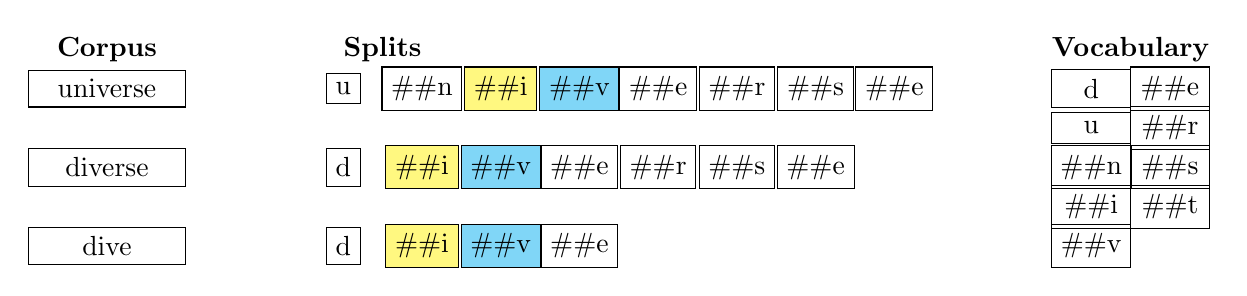
\begin{tikzpicture}

    % Corpus Section
    \node[font=\bfseries] at (0, 0) {Corpus};
    \node[draw, minimum width=2cm, align=center] at (0, -0.5) {universe};
    \node[draw, minimum width=2cm, align=center] at (0, -1.5) {diverse};
    \node[draw, minimum width=2cm, align=center] at (0, -2.5) {dive};
    
    % Splits Section
    \node[font=\bfseries] at (3.5, 0) {Splits};
    % Row 1
    \node[draw] at (3, -0.5) {u};
    \node[draw] at (4, -0.5) {\#\#n};
    \node[draw, fill=yellow!50] at (5, -0.5) {\#\#i};
    \node[draw, fill=cyan!50] at (6, -0.5) {\#\#v};
    \node[draw] at (7, -0.5) {\#\#e};
    \node[draw] at (8, -0.5) {\#\#r};
    \node[draw] at (9, -0.5) {\#\#s};
    \node[draw] at (10, -0.5) {\#\#e};
    % Row 2
    \node[draw] at (3, -1.5) {d};
    \node[draw, fill=yellow!50] at (4, -1.5) {\#\#i};
    \node[draw, fill=cyan!50] at (5, -1.5) {\#\#v};
    \node[draw] at (6, -1.5) {\#\#e};
    \node[draw] at (7, -1.5) {\#\#r};
    \node[draw] at (8, -1.5) {\#\#s};
    \node[draw] at (9, -1.5) {\#\#e};
    % Row 3
    \node[draw] at (3, -2.5) {d};
    \node[draw, fill=yellow!50] at (4, -2.5) {\#\#i};
    \node[draw, fill=cyan!50] at (5, -2.5) {\#\#v};
    \node[draw] at (6, -2.5) {\#\#e};
    
    % Vocabulary Section
    \node[font=\bfseries] at (13, 0) {Vocabulary};
    \node[draw, minimum width=1cm] at (12.5, -0.5) {d};
    \node[draw, minimum width=1cm] at (13.5, -0.5) {\#\#e};
    \node[draw, minimum width=1cm] at (12.5, -1) {u};
    \node[draw, minimum width=1cm] at (13.5, -1) {\#\#r};
    \node[draw, minimum width=1cm] at (12.5, -1.5) {\#\#n};
    \node[draw, minimum width=1cm] at (13.5, -1.5) {\#\#s};
    \node[draw, minimum width=1cm] at (12.5, -2) {\#\#i};
    \node[draw, minimum width=1cm] at (13.5, -2) {\#\#t};
    \node[draw, minimum width=1cm] at (12.5, -2.5) {\#\#v};
    
    \end{tikzpicture}
 
    \caption[Example of one token learner step in WordPiece]{Example of one
    token learner step in WordPiece. The corpus consists of \textit{universe},
    \textit{diverse}, and \textit{dive}. New tokens are formed by merging the
    most likely pair of uni-grams.}    
    \label{fig:wordpiece}
\end{figure}

Fig.~\ref{fig:wordpiece} shows one iteration of the WordPiece tokenization
algorithm on a small corpus. The vocabulary is initialized by taking all single
words and splitting them into so-called \textit{uni-grams}, i.e. single
characters. WordPiece uses special \# symbols in tokens to denote the word does
not begin with these tokens or \textit{word pieces}, which is how the algorithm
refers to tokens. Then the likelihood of all possible pairs of uni-grams is
calculated using the following formula:

\begin{equation}
    \mathrm{likelihood} = \frac{\mathrm{freq\ of\ pair}}{\mathrm{freq\ of\ first\ symbol} 
    \cdot \mathrm{freq\ of\ second\ symbol}}
\end{equation}

In our example, the pair \texttt{(\#\#i, \#\#v)} maximizes the likelihood of the
entire corpus with a value of $\frac{3}{3 \cdot 3} = 0.33$. The pair of
uni-grams with the highest likelihood is then replaced in the corpus with the
merged bi-gram \texttt{\#\#i\#\#v} and added to the vocabulary. The process is
repeated while also taking into account the newly added word piece until the
desired vocabulary size is reached. The authors also propose using the increase
of likelihood as a stopping criterion to prevent the algorithm from merging too
many word pieces. WordPiece specifies the target vocabulary size as the stopping
criterion for the tokenization algorithm, whereas BPE uses the number of
performed merge rules. A vocabulary of 8,000 to 32,000 word pieces is typically
used for WordPiece tokenizers.

\section{Language Modeling} \label{sec:lm}

Language modeling is essential to the functioning of many NLP tasks and involves
predicting upcoming words or tokens in a sequence given some preceding context.
Throughout the section, we will discuss the concept of language modeling in
terms of words, but in practice a language model (LM) is computed over tokens
like the BPE and WordPiece subword tokens of Sec.~\ref{subsec:bpe} and
Sec.~\ref{subsec:wordpiece}. To illustrate, given the preceding context
\textit{``Thanks for all the''}, if we wish to determine the likelihood of the
next word being \textit{``food''} we would compute:

\begin{equation*}
    \Pr(\text{food} | \text{Thanks for all the})
\end{equation*}

In other words, LMs enable us to assign a conditional probability to each
possible next word, resulting in a probability distribution across the entire
vocabulary. We can also determine the likelihood of entire sentences $(w_1, w_2,
\ldots, w_n)$ as the product of conditional probabilities by applying the
\textbf{chain rule of probability} \cite{eisenstein2019intro2nlp}:

\begin{align}
    \Pr(w_1, w_2, \ldots, w_n) &= \Pr(w_1) \Pr(w_2 | w_1) \ldots \Pr(w_n | w_1, \ldots, w_{n-1}) \nonumber \\
    &= \prod_{i=1}^{n} \Pr(w_i | w_1, \ldots, w_{i-1})
\end{align}

The goal of language modeling is to learn the probability distribution of words,
modeling their natural sequential ordering in languages. LMs thus capture the
characteristics of a language and are designed to understand as well as generate
human language by learning patterns, structures and relationships between words.

The reason why LMs are so pivotal in NLP lies in the ability to frame many
practical NLP tasks as word prediction problems \cite{radford2018improving}. For
instance, a textual sentiment analysis can be cast as language modeling by
providing the following exemplary context:

\begin{center}
    \texttt{The sentiment of the sentence "I love this movie" is}
\end{center}

and comparing the conditional probabilities of the words \textit{``positive''}
and \textit{``negative''}. The word with the higher probability is then the
predicted sentiment of the sentence. In speech recognition, the LM can help to
determine the more probable sequence given the previous (transcribed) audio
input. The same applies to more complex tasks like text summarization or
question answering. For the latter, we could prime the LM with the question
followed by a special token, e.g. \texttt{A:}, expecting that an answer should
follow. In the case of a simple factual answer, a single word might suffice as
the result. If a longer textual answer is required, the language modeling
approach can be augmented to include the last generated word in the current
conditioning context and repeat the process until a special end of sentence
token \texttt{[EOS]} is generated (refer to Fig.~\ref{fig:lm_generation}). This
is an example of \textbf{autoregressive generation}, a technique that is widely
used in generating text with LMs. The key ability of powerful language models is
their support for very large context windows. This allows them to incorporate
the condition in its entirety, i.e. paragraphs of input and rounds of generated
outputs, resulting in LMs solving a variety of NLP tasks with a high degree of
accuracy.

\begin{figure}[htbp]
    \centering
    % Source: https://github.com/rodgzilla/talk-slides/blob/master/deep_learning/transformer_language_model/figures/language_modeling.tex
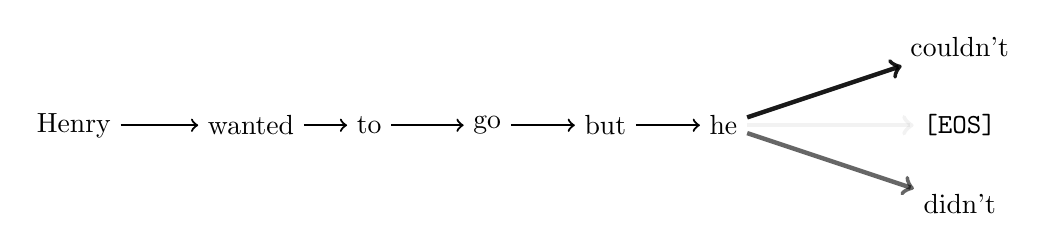
\begin{tikzpicture}[xscale = 1.5]
    \node (W1) at (-.5, 0) {
      Henry
    };
  
  
    \node (W2) at (1, 0) {
      wanted
    };
  
    \node (W3) at (2, 0) {
      to
    };
  
    \node (W4) at (3, 0) {
      go
    };
  
    \node (W5) at (4, 0) {
      but
    };
  
    \node (W6) at (5, 0) {
      he
    };
  
    \node (W8) at (7, 1) {
      couldn't
    };
  
    \node (W9) at (7, 0) {
      \texttt{[EOS]}
    };
  
    \node (W10) at (7, -1) {
      didn't
    };
  
    \draw[thick, ->] (W1) -- (W2);
    \draw[thick, ->] (W2) -- (W3);
    \draw[thick, ->] (W3) -- (W4);
    \draw[thick, ->] (W4) -- (W5);
    \draw[thick, ->] (W5) -- (W6);
    \draw[ultra thick, ->, opacity = 0.9] (W6) -- (W8);
    \draw[ultra thick, ->, opacity = 0.05] (W6) -- (W9);
    \draw[ultra thick, ->, opacity = 0.6] (W6) -- (W10);
  \end{tikzpicture}

    \caption[Example of autoregressive generation with a language model]{Example
    of autoregressive generation with a language model. Each arrow represents
    the sequential prediction of the next word in the sentence. The arrow
    thickness in the final step indicates the probability of the to be predicted
    word.} 
    \label{fig:lm_generation}
\end{figure}

Over the course of several key developments in the history of language modeling,
various types of LMs have been introduced. The first stage was characterized by
simple statistical methods, such as the n-gram model \cite{brown1992class}. This
model was effective for small datasets but struggled with larger contexts. The
second stage saw the introduction of neural networks to NLP, with the
development of the LSTM \cite{hochreiter1997long}. This model is a type of
recurrent neural network (RNN), which allowed the model to maintain information
over longer sequences for more advanced language understanding tasks.
Subsequently, the authors of \cite{dai2015semi} demonstrated that language
modeling could lead to deep language understanding. These previous studies led
to the introduction of the Transformer architecture proposed in
\cite{vaswani2017attention}, which replaced recurrent parts with
\textbf{self-attention} mechanisms. We will introduce this architecture in
detail in Sec.~\ref{sec:transformers}.

\subsubsection{Large Language Models}
The idea to draw knowledge from vast amounts of text data is referred to as
\textbf{pre-training}. Research has shown that scaling up models in terms of
parameter as well as pre-training data size has stretched the models' capability
on a wide range of tasks, particularly \textit{generative} tasks
\cite{min2023recent}. Attributed to their large size, these language models have
thus been coined Large Language Models (LLMs). Unlike traditional deep learning
models, LLMs are very large deep learning models with billions of parameters
trained on massive bodies of text totaling hundreds of gigabytes while using
unsupervised learning objectives. 

LLMs have a high capability of zero or \textbf{few-shot learning}, meaning that
they can adapt well to many downstream tasks by being presented with few
examples, without the need for labeled training data or additional model
modifications \cite{brown2020language}. Conversely, another technique when
adapting LMs to a specific domain, dataset or task is called
\textbf{fine-tuning}, in which we continue training the LM on relevant data.
Various fine-tuning methods exist, depending on which parameters are updated
using the fine-tuning data: all parameters, a subset of parameters, or only
those parameters associated with specific additional circuitry. For the latter,
continued training is often performed \textit{supervised}, since in that case
the fine-tuning data is labeled with the desired output, e.g. class for text
classification. The underlying concept of fine-tuning is that during the
pre-training phase, the LM develops a robust understanding of word meanings,
which then facilitates easier adaptation (or \textit{fine-tuning}) to specific
downstream language tasks. This pretrain-finetune paradigm exemplifies what is
known as \textbf{transfer learning} in machine learning: the process of
acquiring knowledge from one task or domain and subsequently
\textit{transferring} it to solving new tasks \cite{durrani2021transfer}.

These advantages have attracted academia and industry to research and develop
LLMs. In particular, OpenAI introduced its groundbreaking GPT models
\cite{radford2019gpt2, brown2020language, achiam2023gpt}, which serve as the
base for the widely popular chatbot ChatGPT \cite{openai2023chatgpt}. Meta
focused on model accessibility and efficiency with LLaMA
\cite{touvron2023llama1} and its successors \cite{touvron2023llama2,
dubey2024llama3}, while Google prioritized multimodal capabilities with the
Gemini models \cite{rohan2023gemini, georgiev2024gemini}.

\subsection{Masked Language Modeling}

Masked Language Modeling (MLM) is an extension of the language modeling approach
we introduced earlier. A LM trained with this pre-training objective aims to
predict missing words in a sentence, which are randomly selected words that are
replaced with a special \texttt{[MASK]} token. Consider the example in
Tab.~\ref{tab:mlm_example}: Instead of predicting the most likely next word,
here the LM is tasked to predict the masked word \textit{plays} given the rest
of the sentence.

\begin{table}[htb]
    \centering
    \begin{tabular}{p{0.45\textwidth} p{0.45\textwidth}}
        \toprule
        \textbf{Original Sentence} & \textbf{Masked Sentence} \\
        \midrule
        The child plays in the park. & The child \texttt{[MASK]} in the park. \\
        \bottomrule
    \end{tabular}
    \caption{Example sentence for Masked Language Modeling}
    \label{tab:mlm_example}
\end{table}

More precisely, for each masked word we hope that the model computes probability
distributions over the vocabulary that assign maximum likelihood to the
respective missing word. In order to efficiently predict missing words, MLM
incorporates information from the whole sentence, i.e. both left and right
context of the masked word. This usage of \textbf{bidirectional} context differs
from the traditional \textit{unidirectional} language modeling limited to the
left context of past words. While the traditional approach largely focuses on
learning local dependencies between words, MLM facilitates the understanding of
global dependencies and long-range relationships between words in texts
\cite{jurafsky2025slp}. 

This method can be applied to various techniques that modify the training input
and require the model to reconstruct the original version. In addition to
masking, other examples of such modifications include replacing, reordering,
deleting, or adding extra elements to the training text. The technique is known
as \textbf{denoising}, where noise is introduced to the input and the model’s
task is to eliminate the noise.

\subsubsection{Whole Word Masking} \label{subsec:wwm}
As mentioned, we have limited the discussion of language modeling and MLM to the
word level. However, most contemporary tokenizers use subword tokenization.
Whole Word Masking (WWM) addresses this discrepancy by masking on the word level
instead of the individual subword token level. This is achieved by masking all
subword tokens belonging to a word if one of the subwords is masked. 

\begin{table}[htb]
    \centering
    \begin{tabular}{p{0.9\textwidth}}
        \toprule
        \textbf{Original tokenized Sentence:} \\
        The cat is sleep \#\#ing on the mat. \\
        \midrule
        \textbf{Standard MLM:} \\
        The cat is \texttt{[MASK]} \#\#ing on the mat. \\
        \midrule
        \textbf{Whole Word Masking (WWM):} \\
        The cat is \texttt{[MASK]} \texttt{[MASK]} on the mat. \\
        \bottomrule
    \end{tabular}
    \caption{Comparison of standard MLM and Whole Word Masking}
    \label{tab:wwm_example}
\end{table}

In the example given in Tab.~\ref{tab:wwm_example}, the word
\textit{``sleeping''} is split by the tokenizer into the subwords
\textit{``sleep''} and \textit{``\#\#ing''}. During training, only one of the
subwords is masked, diluting the challenge for the model to predict the original
token. With WWM, the entire word is masked, which forces the model to
reconstruct the original word from its surrounding context. By eliminating the
simplest situations, the authors of \cite{chan2020german} have shown that WWM
enhances the training signal for LMs, which results in an improvement in task
performance.

\subsection{Next Sentence Prediction}

While masked language modeling concentrates on predicting words based on their
contextual surroundings to generate meaningful word-level representations,
another crucial aspect of language modeling involves understanding the
relationships between sentence pairs. This is essential for various applications
such as paraphrase detection (identifying if two sentences convey similar
meanings), textual entailment (determining if the meanings of two sentences
support or contradict each other), and discourse coherence (assessing if two
consecutive sentences form a coherent narrative).

Next Sentence Prediction (NSP) is another pre-training objective for LMs,
allowing them to capture the knowledge required for these applications. The task
involves predicting whether two sentences are adjacent in the training corpus.
To illustrate, consider the sentence pairs in Tab.~\ref{tab:nsp_examples}. In
this case, we want the model to predict that the first pair of sentences are
consecutive, while the second pair are not.

\begin{table}[htb]
    \centering
    \begin{tabular}{p{0.45\textwidth} p{0.45\textwidth}}
        \toprule
        \textbf{Sentence Pair 1:} & \textbf{Sentence Pair 2:} \\
        \midrule
        The sky is blue. & The sky is blue. \\
        It looks beautiful today. & I love playing the guitar. \\
        \bottomrule
    \end{tabular}
    \caption{Examples of sentence pairs for Next Sentence Prediction}
    \label{tab:nsp_examples}
\end{table}

NSP enables the efficient usage of the unlabeled training corpus in a
self-supervised manner, as pairs of sentences can be easily built from the
corpus. This process helps the model to grasp the nuances of sentence
relationships, thereby enhancing its performance in tasks that require
understanding of the contextual flow, sentence coherence and long-range
dependencies \cite{jurafsky2025slp}. MLM and NSP form the learning framework for
the BERT model, which will be discussed in Sec.~\ref{sec:bert}. 
